\documentclass{article}
\usepackage[a4paper]{geometry}
\geometry{
  a4paper,
  top=40mm,
}
\usepackage[utf8]{inputenc}
\usepackage[english]{babel}
\usepackage{changepage}

\usepackage{graphicx}
\usepackage{wrapfig}
\usepackage{caption}
\captionsetup[figure]{labelformat=empty}

\usepackage{hyperref}
\hypersetup{
  colorlinks=true,
  linkcolor=blue,
  filecolor=magenta,
  urlcolor=cyan,
}

\usepackage{algorithm}
\usepackage{algpseudocode}

\usepackage{amsmath, amssymb, amsfonts, amsthm, fouriernc, mathtools}
\usepackage{microtype}

\usepackage[svgnames]{xcolor}
\definecolor{lightgrey}{rgb}{0.5,0.5,0.5}
\definecolor{grey}{rgb}{0.25,0.25,0.25}
\newcommand{\blackb}{\color{Black} \usefont{OT1}{lmss}{m}{n}}
\newcommand{\lightgreyb}{\color{lightgrey} \usefont{OT1}{lmss}{m}{n}}

\let\bold\textbf
\newcommand\comb[2][^n]{\prescript{#1\mkern-0.5mu}{}C_{#2}}

\usepackage{titlesec}
\usepackage{sectsty}
\sectionfont{\color{lightgrey}}
\subsectionfont{\color{lightgrey}}
\subsubsectionfont{\color{lightgrey}}

\renewcommand\thesection{\Roman{section}}
\renewcommand\thesubsection{\arabic{section}.\arabic{subsection}}
\renewcommand\thesubsubsection{\arabic{section}.\arabic{subsection}.\arabic{subsubsection}}

\usepackage{chngcntr}
\counterwithin*{equation}{section}

\newcommand{\mysection}{
\titleformat{\section} [runin] {\usefont{OT1}{lmss}{b}{n}\color{lightgrey}}
{\thesection} {3pt} {} }

\renewcommand{\theequation}{\arabic{section}.\arabic{equation}}

\usepackage{etoolbox}
\makeatletter
\patchcmd{\@Aboxed}{\boxed{#1#2}}{\colorbox{black!15}{$#1#2$}}{}{}
\patchcmd{\@boxed}{\boxed{#1#2}}{\colorbox{black!15}{$#1#2$}}{}{}
\makeatother

\title{\vspace{-4ex}\lightgreyb Data Structures and Algorithms \\
\lightgreyb Assignment $4$ Solutions}
\author{Ayush Bansal \\
Roll No. 160177}
\date{\vspace{-4ex}}

\newtheorem{theorem}{Theorem}
\newtheorem{corollary}{Corollary}[theorem]
\newtheorem{conjecture}{Conjecture}
\newtheorem{lemma}{Lemma}[section]
\newtheorem{claim}{Claim}[section]
\newenvironment{solution}
  {\begin{proof}[Solution]}
  {\end{proof}}
\AfterEndEnvironment{theorem}{\noindent\ignorespaces}
\renewcommand\thelemma{\arabic{section}.\arabic{lemma}}
\renewcommand\theclaim{\arabic{section}.\arabic{claim}}

\newenvironment{myenv}{\begin{adjustwidth}{1cm}{}}{\end{adjustwidth}}

\begin{document}
\maketitle

\section{Problem 1 Solution}{
  \subsection{Part 1}{
    We are given a \bold{unique path graph} $G$ and we have to comment on the existence of forward, cross and backward edges in the DFS tree $T_v$ of a vertex $v$.
    \begin{figure}[h]
      \begin{minipage}[h]{0.24\textwidth}
        \centering
        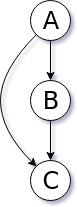
\includegraphics[scale=0.3]{forward}
        \caption{Forward Edge}
      \end{minipage}
      \begin{minipage}[h]{0.24\textwidth}
        \centering
        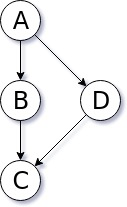
\includegraphics[scale=0.3]{cross}
        \caption{Cross Edge}
      \end{minipage}
      \begin{minipage}[h]{0.24\textwidth}
        \centering
        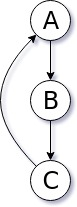
\includegraphics[scale=0.3]{back}
        \caption{Backward Edge}
      \end{minipage}
      \begin{minipage}[h]{0.24\textwidth}
        \centering
        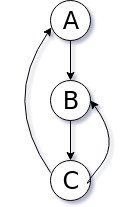
\includegraphics[scale=0.3]{2back}
        \caption{2 Backward Edges}
      \end{minipage}
    \end{figure}
    \newline \bold{Forward Edges}
    \begin{myenv}
      In case of forward edges in the graph, consider the example in the figure above, there are $2$ paths from vertex $A$ to $C$ and thus forward edges are \bold{Not Possible}. \newline
    \end{myenv}
    \bold{Cross Edges}
    \begin{myenv}
      In case of cross edges in the graph, consider the example in the figure above, there are $2$ paths from vertex $A$ to $C$ and thus cross edges are \bold{Not Possible}. \newline
    \end{myenv}
    \bold{Backward Edges}
    \begin{myenv}
      In case of backward edges, consider the example in the figure above, there are no $2$ different paths for any pair of vertices, thus cycles are allowed in the directed graph as backward edges are allowed.
      So, backward edges are \bold{Possible and Allowed}. \newline
    \end{myenv}
    \bold{2 Backward Edges from a single node}
    \begin{myenv}
      In case of 2 backward edges from a single node in the graph, consider the example in the figure above, there are $2$ paths from vertex $C$ to $B$ and thus 2 backward edges from a single node are \bold{Not Possible}.
      \newline Thus, the graph can atmost have $V-1$ back edges (leaving out root vertex).
    \end{myenv}
    \begin{lemma}
      The necessary and sufficient condition for a directed graph $G$ to be a unique path graph is "there shouldn't be any forward or cross edges in the DFS tree $T_v$ of any vertex $v\in V$". 
    \end{lemma}
    \begin{proof}
      Let's assume $G$ is a unique path graph and there is a forward or a cross edge in certain DFS tree $T_v$ for some $v \in V$. \newline
      From the above discussion on the the existence of forward, cross and backward edges in the DFS tree of vertex $T_v$, it is clear that if there is a forward or a cross edge, then the path from a vertex $A$ to a vertex $C$ s.t. $A,C \in V$ will not be unique and thus the graph $G$ will not be a unique path graph which is a \bold{contradiction}. \newline
      Thus, for each $v\in V$, there shouldn't be any forward or cross edge in the DFS tree $T_v$ otherwise, the uniqueness of atleast one path will be lost and the graph $G$ will not be a unique path graph. \newline
      Now, Let's assume that $G$ is not unique path graph and has no forward or cross edges in any DFS tree $T_v$ for all $v\in V$. \newline
      Since $G$ is not a unique path graph, there exist nodes $a,b \in V$ such that there are $2$ different paths from vertex $a$ to vertex $b$.
      If there are $2$ paths from vertex $a$ to $b$ then there will be a DFS tree $T_v$ for some $v\in V$ which will contain a cross or forward edge from vertex $a$ to $b$ leading to \bold{contradiction}. \newline
      Thus, the graph $G$ must be a unique path graph.
    \end{proof}
  }
  \subsection{Part 2}{
    Since any DFS tree $T_v$ of the graph cannot have more than $V-1$ back edges and also the tree edges will be equal to $V-1$, the total number of edges in a unique path graph \bold{$E\leq2V-2$}. \newline
    I will perform a \bold{DFS traversal} taking each node of the graph as source one at a time, if in any DFS tree $T_v$, a forward or a cross edge is found, then the graph is not a unique path graph. \newline
    Following will be the algorithm of \bold{modified DFS} for detecting forward and cross edges.
    \begin{algorithm}
      \caption{DFS Traversal}\label{dfs}
      \begin{algorithmic}[1]
        \Procedure{DFS}{$u$}\Comment{Takes source vertex, color is global array}
          \State $color[u]\gets$GREY\Comment{Grey means vertex \bold{discovered}}
          \ForAll{$v\in Adj[u]$}
            \If{$color[v] = $BLACK}\Comment{If forward or cross edge is found}
              \State $flag\gets false$\Comment{Flag is global Boolean}
              \State \Return
            \ElsIf{$color[v] = $WHITE}\Comment{Move to adjacent undiscovered vertex}
              \State DFS(v)
            \EndIf
          \EndFor
          \State $color[u]\gets$BLACK\Comment{Black means Vertex has \bold{finished} traversal}
        \EndProcedure
      \end{algorithmic}
    \end{algorithm}
    \newline Below will be the algorithm which will call the above procedure and report if the graph is unique path graph or not.
    \begin{algorithm}
      \caption{UniqueOrNot}\label{upg}
      \begin{algorithmic}[1]
        \Procedure{UniqueOrNot}{$Graph$ $G$}\Comment{Returns true if Unique path graph}
          \State $flag\gets true$\Comment{flag will be returned finally}
          \ForAll{$u\in V[G]$}\Comment{Calling DFS for each vertex}
            \If{$flag = false$}
              \State \bold{break}
            \EndIf
            \ForAll{$v\in V[G]$}\Comment{Mark all vertices undiscovered for new dfs}
              \State $color[v]\gets$WHITE\Comment{White means vertex \bold{undiscovered}}
            \EndFor
            \State DFS(u)\Comment{Calling DFS procedure with $u$ as root}
          \EndFor
          \State \Return $flag$\Comment{Flag is set to false within DFS if not unique path graph}
        \EndProcedure
      \end{algorithmic}
    \end{algorithm}
    \newline \bold{Time Complexity}
    \begin{myenv}
      The time complexity of \bold{DFS} is $O(V+E)$ but is reduced to $O(V)$ since $E\leq 2V-2$ (already shown) otherwise we will definitely find a forward edge and algorithm will end. \newline
      The time complexity of \bold{UniqueOrNot} procedure will be $O(V(V+E))$ and since $E\leq 2V-2$, the final complexity will be $O(V^2)$.
    \end{myenv}
  }
}
\newpage
\section{Problem 2 Solution}{
  We are given a set of $N$ boolean variables $X = \{x_1,\dots,x_N\}$ and an expression $E=a_1\wedge a_2 \wedge \dots a_K$ s.t. $a_k = y_i \vee y_j$ where $y_i,y_j$ are literals. \newline
  For the question, $$E = (x_1 \vee x_3) \ \wedge\ (\neg x_1 \vee x_4) \ \wedge\ (x_2 \vee x_3) \ \wedge\ (x_2 \vee \neg x_4)$$
  \subsection{Part 1}{
    We know that $a\vee b \equiv b\vee a$ and $a\vee b \equiv \neg a \Rightarrow b$, so we will have $$a\vee b \equiv (\neg a \Rightarrow b) \wedge (\neg b\Rightarrow a)$$
    Thus, the converted expression $E$ can be written in $2$ forms both of which will be equivalent (one is extended version) as $a\vee b \equiv b\vee a$.
    \begin{align*}
      E = (\neg x_1 \Rightarrow x_3) \ \wedge\ (x_1 \Rightarrow x_4) \ &\wedge\ (\neg x_2 \Rightarrow x_3) \ \wedge\ (\neg x_2 \Rightarrow \neg x_4) \\
      E = (\neg x_1 \Rightarrow x_3) \ \wedge\ (\neg x_3 \Rightarrow x_1) \ \wedge \ (x_1 \Rightarrow x_4) \ \wedge\ (\neg x_4 \Rightarrow \neg x_1) \ &\wedge \ (\neg x_2 \Rightarrow x_3) \ \wedge\ (\neg x_3 \Rightarrow x_2) \ \wedge \ (\neg x_2 \Rightarrow \neg x_4) \ \wedge \ (x_4 \Rightarrow x_2)
    \end{align*}
    For constructing the graph we will choose \bold{boolean variables and their negations} as the Vertex set and the \bold{Implication relations} as the Edge set.
    \begin{itemize}
      \item{2 edges for every clause i.e. $\neg A\rightarrow B$ and $\neg B\rightarrow A$ for clause $A\vee B$.}
      \item{1 node for every Boolean variable involed in the Boolean expression i.e. $A$, $\neg A$, $B$, $\neg B$ etc.}
      \item{So, total $2K$ edges for $K$ distinct clauses and $2N$ vertices for $N$ boolean variables.}
    \end{itemize}
    Following is the graph for the expression $E$, it will have $2N=8$ vertices and $2K=8$ edges.
    \begin{figure}[h]
      \centering
      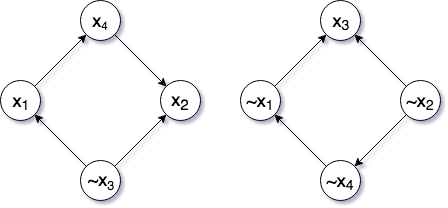
\includegraphics[scale=0.3]{egraph}
    \end{figure}
  }
  \subsection{Part 2}{
    Now, we have got a graph from the expression $E$ and we have to find whether $E$ is satisfiable or not.
    \begin{lemma}
      If both $x_i$ and $\neg x_i$ lie in the same \bold{SCC} (Strongly Connected Component), the CNF (Expression) is \bold{unsatisfiable}, otherwise it is \bold{satisfiable}.
    \end{lemma}
    \begin{proof}
      Consider the following cases of existence of edges which obey the rules of implication (if $A$ then $B$).
      \begin{enumerate}
        \item{Edge $x_i\Rightarrow \neg x_i$ exists, then $x_i$ must be \bold{false} otherwise the statement can't be satisfiable.}
        \item{Edge $\neg x_i\Rightarrow x_i$ exists, then $x_i$ must be \bold{true} otherwise the statement can't be satisfiable.}
        \item{Both edges $\neg x_i\Rightarrow x_i$ and $x_i\Rightarrow \neg x_i$ exist, then the statement is \bold{unsatisfiable}.}
      \end{enumerate}
      Using the fact that a path (SCC) like $a \Rightarrow b \Rightarrow c \Rightarrow a$ in graph will have same truth values for all. \newline
      If there is a path both from $x_i$ to $\neg x_i$ and from $\neg x_i$ to $x_i$, then the expression is \bold{unsatisfiable}. \newline
      The above statement is same as saying that $x_i$ and $\neg x_i$ are part of the same \bold{SCC} (Strongly Connected Component) as there exists a path from $x_i$ to $\neg x_i$ as well as $\neg x_i$ to $x_i$. \newline
      If $x_i$ and $\neg x_i$ do not lie in the same SCC, then it is possible to assign truth values to the variables according to \bold{case 1 \& 2} above and thus, the expression is \bold{satisfiable}.
    \end{proof}
    \noindent\bold{Algorithm to find Satisfiably}:
    \begin{itemize}
      \item{Find all the \bold{SCCs} in the graph using the algorithm studied in class.}
      \item{Check if any SCC contains both a boolean variable and its negation i.e. $x_i$ and $\neg x_i$.}
        \begin{itemize}
          \item{If yes (i.e. it contains both), then report \bold{unsatisfiable}.}
          \item{Else, report \bold{satisfiable}.}
        \end{itemize}
    \end{itemize}
    In case of graph of expression $E$, there is no SCC containing both $x_i$ and $\neg x_i$, thus it is \bold{satisfiable}.
  }
  \subsection{Part 3}{
    We are given a \bold{satisfiable} expression $E$ and I have to assign truth values to the variables in $X$.
    \begin{lemma}
      The graph formed by merging all vertices in an \bold{SCC} (Strongly Connected Component) into a single vertex and doing it for all SCCs is a \bold{Directed Acyclic Graph}.
    \end{lemma}
    \begin{proof}
      Assume graph formed by mentioned process is not a \bold{DAG}, then there is a cycle containing atleast $2$ vertices. \newline
      Since these vertices represent $2$ different SCCs and there is a path leading from SCC1 to SCC2 and vice versa, thus there will be a path from each and every vertex of SCC1 to SCC2 and also from SCC2 to SCC1 and thus, they will not remain different SCCs anymore which is a contradiction to our original graph. \newline
      Thus, the graph formed must be a Directed Acyclic Graph.
    \end{proof}
    \noindent Given an expression $E$, the complete algorithm for assigning truth values to the variables in $X$ is
    \begin{itemize}
      \item{Build a directed graph using each \bold{SCC} as a vertex and the edges from this SCC to others as edges of this graph, basically merging all the vertices in an SCC into one.}
      \item{Perform a \bold{topological sort} on the above newly formed graph (already proved it is a \bold{DAG}).}
      \item{Assign truth values to each \bold{SCC} in order of topological sort \bold{till all the boolean variables have an assigned truth value} as follows.}
        \begin{itemize}
          \item{If all the boolean variables in an SCC are unassigned, assign all the truth value of \bold{TRUE} and their negations the truth value of \bold{FALSE}.}
          \item{If a boolean variable in SCC is assigned some value, then assign the same value to the rest of the variables in that SCC and give the opposite value to negations.}
          \item{Stop when all the boolean variables in $X=\{x_1,\dots,x_n\}$ are assigned.}
        \end{itemize}
    \end{itemize}
    Using the above algorithm, there could be $2$ possible orderings of the SCC graph formed by expression $E$, so their corresponding truth values will be:
    \begin{center}
    \begin{tabular}{|| c | c ||}
      \hline
      \bold{Topological - Ordering} & \bold{Truth Values} \\ [0.5ex]
      \hline \hline
      $\neg x_3,x_1,x_4,x_2,\neg x_2,\neg x_4,\neg x_1,x_3$ & $x_3$ -> False \\
      & $x_1,x_2,x_4$ -> True \\
      \hline
      $\neg x_2,\neg x_4, \neg x_1, x_3, \neg x_3, x_1, x_4, x_2$ & $x_3$ -> True \\
      & $x_1, x_2,x_4$ -> False \\
      \hline
    \end{tabular}
    \end{center}
    Taking example of \bold{first} ordering:
    \begin{itemize}
      \item{Assign $\neg x_3$ -> True, and $x_3$ -> False.}
      \item{Assign $x_1$ -> True, and $\neg x_1$ -> False.}
      \item{Assign $x_4$ -> True, and $\neg x_4$ -> False.}
      \item{Assign $x_2$ -> True, and $\neg x_2$ -> False.}
      \item{Stop as all variables have been assigned.}
    \end{itemize}
  }
}
\end{document}
